\section{Echtzeitbetriebssystem}

\subsection{Aufgaben}
\begin{itemize}
	\item Ausführung der Benutzerprogramme
	\item Verteilung der Betriebsmittel
	\item evtl. Steuerung, Überwachung
	\item Standartisierter Zugriff (virtuelle Maschine)
\end{itemize}

\subsection{Anforderungen: Prozessmanagement}
\begin{itemize}
	\item Zeitverhalten
	\begin{itemize}
		\item Schnelligkeit
		\item Bei einem RTOS insbesondere die Realisierung kurzer Antwortzeiten
		\item Zeitlicher Determinismus (z.B. Speicherverwaltung/Garbage Collection ist
	\end{itemize}
	
	\item Geringer Ressourcenverbrauch
	\begin{itemize}
		\item Hauptspeicher
		\item Prozessorzeit
	\end{itemize}
	
	\item Zuverlässigkeit und Stabilität
	\begin{itemize}
		\item Programmfehler dürfen Betriebssystem und andere Programme nicht beeinflussen
	\end{itemize}
	
	\item Sicherheit
	\begin{itemize}
		\item Dateischutz, Zugangsschutz
	\end{itemize}
	
	\item Portabilität, Flexibilität und Kompatibilität
	\begin{itemize}
		\item Erweiterbarkeit von Systemen
		\item Einhalten von Standards (z.B. POSIX)
		\item Möglichkeit, für andere BS geschriebene Programme zu portieren
	\end{itemize}
	
	\item Skalierbarkeit
	\begin{itemize}
		\item Hinzunehmen oder Weglassen von BS-Komponenten ermöglichen
		\item Geringer (Programm-, Daten-)Speicherbedarf („Footprint“)
		\item Komfort und umfassende Funktionalität bei großen Anwendungen
	\end{itemize}
\end{itemize}

\subsection{Determinismus}
\begin{itemize}
	\item Scheduling
	\item IPC und Synchronisation
	\item Speichermanagement: kein Swapping oder Garbage Colleciton
\end{itemize}

\subsection{Unterbrechbarkeit}
\begin{itemize}
	\item Software Interrupt (Betriebssystem-Dienst Anfordern: \underline{Systemcall})
	\item Hardware Interrupt (Hardware fordert Dienste)
	\item $\Rightarrow$ Präemtives Scheduling $\Rightarrow$ \underline{TCB}
\end{itemize}

\subsubsection{Task Controll Block}
\begin{itemize}
	\item Priorität
	\item Maschinenzustand (Register, Stack, ...)
	\item Task-Zustand (+Bedingungen, auf die die Task wartet)
	\item Zeit-Quantum („erzeugte Prozessorlast“; Summe, in letzter Zeiteinheit)
	\item Verwaltungsdaten für Betriebsmittel (Filedeskriptoren,...)
	\item Speicherabbildungstabellen virtueller Speicher (Prozessadressraum) ->
realer Speicher (code, data, stack)
\end{itemize}

\subsubsection{Lightweight Processes}
Minimierung des Kontextwechsels (nur \underline{Stack} und \underline{PC} werden separiert)

\subsection{Speicherverwaltung}
\subsubsection{MMU}
\begin{itemize}
	\item Speicherschutz
	\item Adressumsetzung $\Rightarrow$ \underline{Shared Libraries}
	\item mit Hardware realisiert
\end{itemize}

\subsubsection{Keine MMU}
\begin{itemize}
	\item Alle Programme zur Link-Zeit bekannt $\Rightarrow$ \underline{zuordnen von Adressbereichen und Sprungadressen}
	\item Loader: Ersetzt Adressen zur Lade-Zeit eines Programms
	\item Position Independent Code
\end{itemize}

\subsection{IO-System}
(\textbf{Unix}: Geräte werden \underline{im Dateisystem} abgebildet) \\
$\Rightarrow$ Zugriffswunsch bei OS anmelden $\rightarrow$ Zugriffsrechte $\rightarrow$ Filedescriptor

\subsubsection{Kernelmode}
\begin{itemize}
	\item Einheitlicher zugriff
	\item Kapselung
	\item Sicherheit
\end{itemize}

\subsubsection{Systemcall}
\begin{figure}[h!]
	\begin{center}
		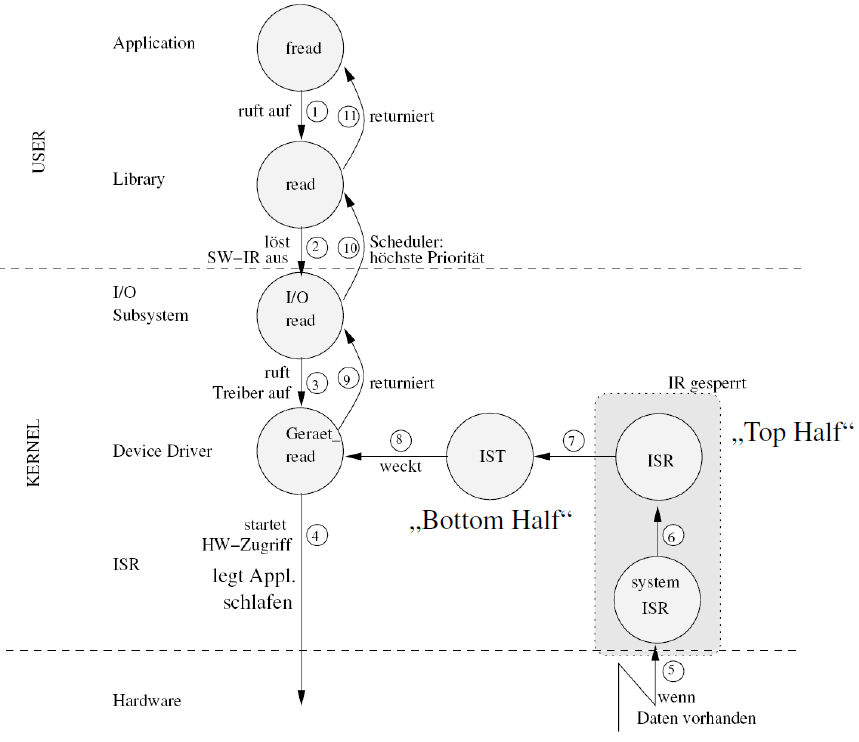
\includegraphics[width=.75\linewidth]{pics/syscall}
		\caption{Ablauf: Systemcall}
	\end{center}
\end{figure}

\subsubsection{Latenzzeiten}
\begin{figure}[h!]
	\begin{center}
		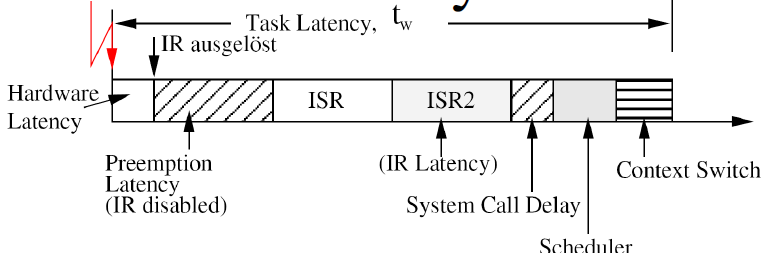
\includegraphics[width=.75\linewidth]{pics/latency}
		\caption{IO Latenzzeiten}
	\end{center}
\end{figure}

\subsubsection{Dateizugriff}
\begin{itemize}
	\item Synchronous IO (Implizites Warten) \\
	\underline{Unblock wenn}:
	\begin{itemize}
		\item Antwort des Geräts
		\item Fehlerzustand
		\item Signal an Task
	\end{itemize}
	
	\item Asynchronous IO (Explitizes Warten) \\
	\underline{kein blocking, sondern}:
	\begin{itemize}
		\item callback
		\item polling
		\item Signal an Task
	\end{itemize}
	
	\item Asynchronous: Probleme
	\begin{itemize}
		\item Parallelität von Task aus garantieren
		\item Applikationsende $\Rightarrow$ \underline{OS-Verwaltungsaufwand}
	\end{itemize}
\end{itemize}
